\section{Auswertung}
\label{sec:Auswertung}
Der Versuch wird, wie in \autoref{sec:Durchführung} aufgebaut und durchgeführt.
\subsection{Bestimmung der Weglänge}
\label{subsec:Weglänge}
Im Folgenden wird die mittlere Weglänge bei verschiedenen Temperaturen bestimmt. Dazu wird mit \autoref{eqn:psät} der Sättigungsdampfdruck $p_{s\ddot{a}t}$ bei den gemessenen 
Temperaturen bestimmt. Danach wird $\bar{\omega}$ mit der \autoref{eqn:Weglänge} bestimmt. Alle Werte werden in die \autoref{tab:Weglänge} eingetragen.
\begin{table}[H]
  \centering
  \caption{Gemsesene und bestimmte Werte für die Wellenlänge.}
  \label{tab:Weglänge}
  \sisetup{table-format=2.2}
  \begin{tabular}{S[table-format=3.2] S[table-format=2.3] S[table-format=1.4] S[table-format=4.1]}
  \toprule
  {Temperaturen $T / \si{\kelvin}$} & {Sättigungsdampfdruck $p_{s\ddot{a}t} / \si{\milli\bar}$} & {mittlere Weglänge $\bar{\omega} / \si{\centi\meter}$} & {Verhältnis $\frac{a}{\bar{\omega}}$}\\
  \midrule
    296.45   & 0.005 & 0.6241 & 1602.2 \\
    416.15  & 3.669 & 0.0008  & 1265.2 \\
    442.15  & 9.695 & 0.0003  & 3342.9 \\
    452.15  & 13.674 & 0.0002 & 4715.2 \\
  \bottomrule
  \end{tabular}
\end{table}
Das Verhältnis $\frac{a}{\bar{\omega}}$ wird auch in \autoref{tab:Weglänge} eingetregen mit $a = \qty{1}{\centi\meter}$. 
%T =  [296.45 416.15 442.15 452.15]
%psät=  [4.64657855e-03 3.66913288e+00 9.69451481e+00 1.36740660e+01]
%w =  [6.24115136e-01 7.90377480e-04 2.99138230e-04 2.12080298e-04]
%aw =  [1.60226846e+00 1.26521823e+03 3.34293614e+03 4.71519518e+03]
%Ende der Weglänge

\subsection{Integrale und differentielle Energieverteilung}
\label{subsec:Energieverteilung}

Tiefpunkt für $T_1$ bei $\qty{8.25}{\volt}$ und $T_2$ bei $\qty{1.29}{\volt}$.

%Ende der Energieverteilung

\subsection{Franck-Hertz-Kurve} % (fold)
\label{sub:Franck-Hertz-Kurve}
Die Franck-Hertz-Kurve wird bei zwei Temperaturen untersucht und aufgezeichnet (siehe \autoref{fig:plot3} und \autoref{fig:2.jpeg}). 
Die Temperaturen liegen bei $T_3= \qty{169}{\celsius}$ und bei $T_4= \qty{179}{\celsius}$.

\begin{figure}
  \centering
  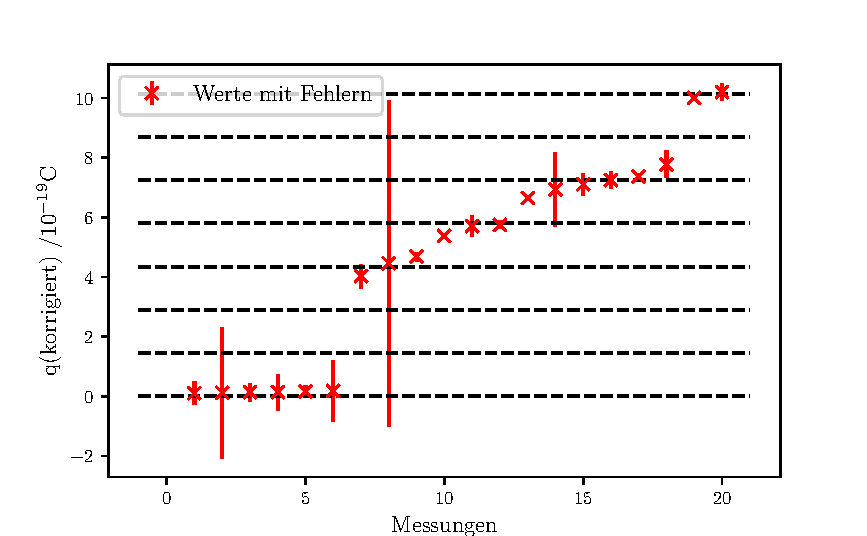
\includegraphics[width=\textwidth]{plot3.pdf}
  \caption{Franck-Hertz-Kurve bei $T_3$ und $T_4$.}
  \label{fig:plot3}
\end{figure}


% subsection Franck-Hertz-Kurve (end)





